% Chapter Template

\chapter{Ensayos y resultados} % Main chapter title

\label{Chapter4} % Change X to a consecutive number; for referencing this chapter elsewhere, use \ref{ChapterX}

%----------------------------------------------------------------------------------------
%	SECTION 1
%----------------------------------------------------------------------------------------
Esta sección presenta los diferentes prototipos realizados para determinar la viabilidad de cada una de las funcionalidades provistas, la metodología de desarrollo, testing, y finalmente los entregables finales del trabajo.

\section{Proceso de desarrollo y aseguramiento de calidad}
\label{sec:pruebasHW}

Para el proceso de desarrollo se utilizó TDD (Test Driven Development) con CMock, Ceedling y Unity como frameworks para abordar esto. Para la construcción de los casos de pruebas se utilizó Control Flow Test como técnica de caja blanca a fin de diseñar los tests unitarios y de integración. 
Adicionalmente, se configuró el entorno de desarrollo basado en Docker, por lo que se extiende la imagen de Espressif y se agregó el conjunto de utilidades ESP-IDF Components como parte de la misma. Luego de versionar esta imagen en el \textit{Docker Registry} utilizado se configuró el servidor de integración continua para ejecutar las compilaciones usando esta imagen por cada push realizado.
En la siguiente imagen se puede apreciar la infraestructura implementada para abordar el ciclo de desarrollo y despliegue. 


[pendiente imagen]

\section{Prototipos de los diferentes modulos}
\label{sec:pruebasHW}

Se suigio una metodologia basada en lograr prototipar las funcionalidades de los diferentes modulos independientes para luego integrarlas todas juntas en un prototipo integrador. En las siguientes secciones se explican los diferentes prototipos realizados.

\subsection{Prototipo de funcionalidad de medición de temperatura y humedad}

Se 



\subsection{Prototipo de funcionalidad de medición de presión}
Para el desarrollo de este prototipo se utilizó el framework ESP-IDF y la biblioteca de código ESP-IDF Components que provee el soporte para gestionar el BMP280. A continuación se puede apreciar el conexionado del prototipo en la figura \ref{fig:conexionado_bmp280} y los detalles de sus pines en la tabla \ref{tab:conexionado_bmp280}.

\vspace{0.5cm}    
\begin{table}[h]
\centering
\caption[Conexionado BMP280]{Conexionado BMP280}
\begin{tabular}{l c }
\toprule
\textbf{Nombre lógico} &  \textbf{Pin GPIO}\\
\midrule
 BMP SDA & 18 \\
 BMP280 SCL & 19  \\
\bottomrule
\hline
\end{tabular}
\label{tab:conexionado_bmp280} 
\end{table}
    
\vspace{0.5cm}    
\begin{center}
  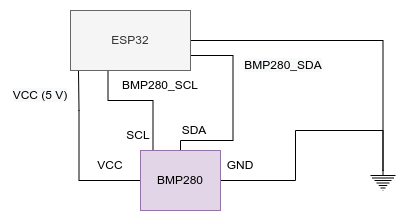
\includegraphics[scale=1]{conexionado_bmp280}
    \captionof{figure}{Conexionado BMP280.}
    \label{fig:conexionado_bmp280}
\end{center}




\subsection{Prototipo de funcionalidad de medición de valor de luminosidad}
Para el desarrollo de este prototipo se utilizó el siguiente conexionado y la biblioteca de código ADC provista por ESP-IDF. A continuación se puede apreciar el conexionado del prototipo en la figura \ref{fig:conexionado_fotoresistor} y los detalles de sus pines en la tabla \ref{tab:conexionado_fotoresistor}.

\vspace{0.5cm}    
\begin{table}[h]
\centering
\caption[Conexionado fotorresistor]{Conexionado fotorresistor}
\begin{tabular}{l c c}
\toprule
\textbf{Nombre lógico} & \textbf{Pin ADC} & \textbf{Pin GPIO}\\
\midrule
ADC Fot pin & channel 0 - unit 2 & 4\\
\bottomrule
\hline
\end{tabular}
\label{tab:conexionado_fotoresistor}
\end{table}


\vspace{0.5cm}
\begin{center}
  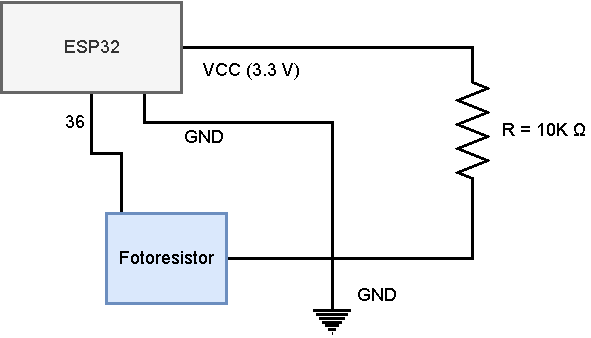
\includegraphics[scale=1]{conexionado_fotoresistor}
    \captionof{figure}{Conexionado fotorresistor.}
    \label{fig:conexionado_fotoresistor}
    
\end{center}
\subsection{Prototipo de funcionalidad de obtencion de valores analogicos del joystick}
Para el desarrollo de este prototipo se utilizó el siguiente conexionado y la biblioteca de código ADC provista por ESP-IDF. A continuación se puede apreciar el conexionado del prototipo en la figura \ref{fig:conexionado_joystick} y los detalles de sus pines en la tabla \ref{tab:conexionado_joystick}.


\vspace{0.5cm}
\begin{table}[h]
\centering
\caption[Conexionado joystick]{Conexionado joystick}
\begin{tabular}{l c c}
\toprule
\textbf{Nombre lógico} & \textbf{Pin ADC} & \textbf{Pin GPIO}\\
\midrule
ADC X & channel 1 - unit 2 & 0 \\
ADC Y & channel 7 - unit 1 & 35 \\
\bottomrule
\hline
\end{tabular}
\label{tab:conexionado_joystick}
\end{table}

\vspace{0.5cm}

\begin{center}
  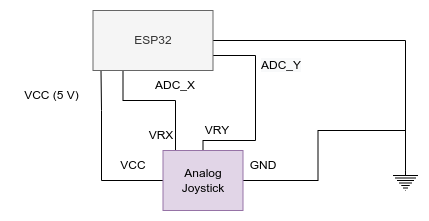
\includegraphics[scale=1]{conexionado_joystick}
    \captionof{figure}{Conexionado joystick.}
    \label{fig:conexionado_joystick}
    

\end{center}

\subsection{Prototipo de funcionalidad de presentación de display}
 

\subsection{Prototipo de funcionalidad de control de motores DC}


...

\section{Tests de los diferentes módulos}
\label{sec:pruebasHW}

...

\section{Tests del producto final}
\label{sec:pruebasHW}

...

\section{Reportes de testing}
\label{sec:pruebasHW}

...

\section{Verificacion y validacion del producto}
\label{sec:pruebasHW}

...

\section{Documentacion del producto }
\label{sec:pruebasHW}

...



